\documentclass[10pt, a4paper]{article}

% Text packages
\usepackage[french]{babel}
\usepackage[utf8]{inputenc}
\usepackage{lmodern} % Latin founts

% Fonts packages
\usepackage{ifxetex}
\ifxetex
    \usepackage{fontspec}
    \setmainfont{OpenDyslexic}
\else
    \usepackage[T1]{fontenc}
\fi

% Math fonts
\usepackage{amsmath}
\usepackage{amsfonts}
\usepackage{latexsym}

% Theorem fonts
\usepackage{amsthm}

% Title import
\usepackage{authoraftertitle}

% Clickable link
\usepackage{hyperref}
\hypersetup{
    colorlinks=true,
    citecolor=blue,
    filecolor=black,
    linkcolor=black,
    urlcolor=blue
}

% Image side by side
\usepackage{subcaption}

% Text color
\usepackage{xcolor}

\usepackage{xspace}

% Image
\usepackage{graphicx}
\graphicspath{ {./images/} }
\usepackage{bookmark}

% Code import
\usepackage{minted}
\usemintedstyle{emacs} % borland

\title{PaP}
\author{BERASATEGUY Tanguy, GOEDEFROIT Charles}

\begin{document}

\begin{titlepage}
	\centering
    \ {} % important
	\vfill
	\vspace{1cm}
	{\scshape\LARGE\MyTitle\par}
	\vspace{0.5cm}
	{\huge\bfseries Projet : rapport2\par}
	\vspace{0.5cm}
	{\Large 4TIN804U\par}
	\vspace{1cm}
	\MyAuthor
	\vfill
	{\large2021-2022\par}
\end{titlepage}

\newpage

\tableofcontents

\newpage

\section{ILP optimization (4.1)}

On a fait les modifications :

Pour \emph{ssandPile\_do\_tile\_opt()} on a retiré les appels à \em{table(out, i, j)}
pour passer par une varaible intermediaire result. Cette modification permet au compilateur
de vectoriser car il peut maintenant facilement voir que les différentes lignes peuvent être
calculés en parallels.\\

Nous avons modifié ces lignes :
\inputminted[
    frame=lines,
    framesep=2mm,
    baselinestretch=1.2,
    fontsize=\footnotesize,
    linenos,
    firstline=1,
    lastline=25
]{diff}{codes/sync_do_tile_opt.c}

Le code de la fonction final :
\inputminted[
    frame=lines,
    framesep=2mm,
    baselinestretch=1.2,
    fontsize=\footnotesize,
    linenos,
    firstline=27,
    lastline=45
]{c}{codes/sync_do_tile_opt.c}

Nous avons verifié et on obtient le même résultats et le même nombre d'iterations (69190)
avec la version par défaut et la version opt.\\
\begin{figure}[H]
    \centering
    \begin{subfigure}{.4\textwidth}
        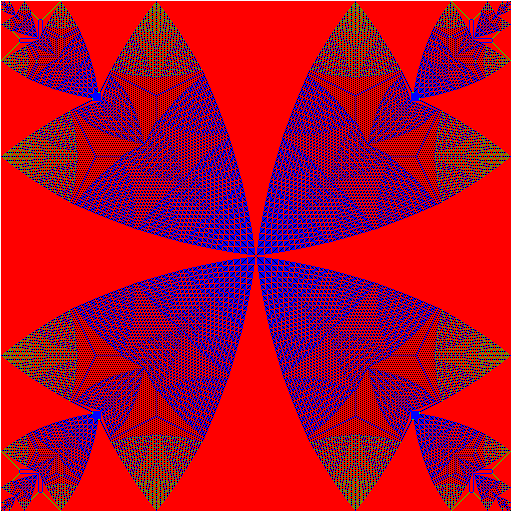
\includegraphics[width=1\linewidth]{dump-ssandPile-seq-dim-512-iter-69190_default}
        \caption{\small{avec do\_tile\_default}}
        \label{fig:ssandPile_default}
    \end{subfigure}
    \begin{subfigure}{.4\textwidth}
        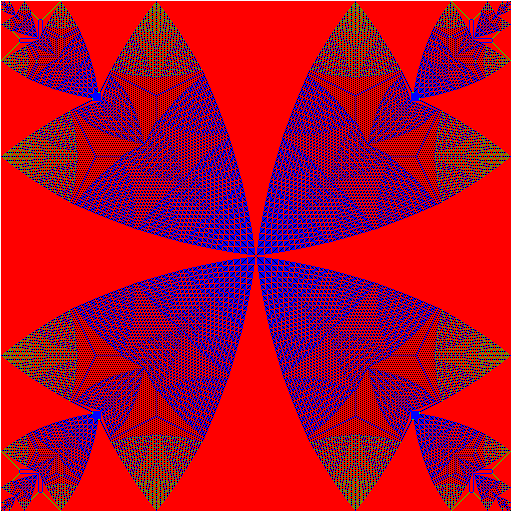
\includegraphics[width=1\linewidth]{dump-ssandPile-seq-dim-512-iter-69190_opt}
        \caption{\small{avec do\_tile\_opt}}
        \label{fig:ssandPile_opt}
    \end{subfigure}
    \caption{Verification du résultats pour ssandPile}
\end{figure}

Le gain de performance est de $2.37$ car $\frac{178812}{75408}$
\\[0.5cm]

Pour \emph{asandPile\_do\_tile\_opt()} on a retiré les appels à \em{atable(i, j)} pour passer par une variable intermédiaire result. Cette modification permet au compilateur
de vectoriser car il peut maintenant facilement voir que les différentes lignes peuvent être calculés en parallele.

Nous avons modifié ces lignes :
\inputminted[
    frame=lines,
    framesep=2mm,
    baselinestretch=1.2,
    fontsize=\footnotesize,
    linenos,
    firstline=1,
    lastline=24
]{diff}{codes/async_do_tile_opt.c}

Le code de la fonction final :
\inputminted[
    frame=lines,
    framesep=2mm,
    baselinestretch=1.2,
    fontsize=\footnotesize,
    linenos,
    firstline=26,
    lastline=46
]{c}{codes/async_do_tile_opt.c}

Nous avons verifié et on obtient le même résultat et le même nombre d'iterations (34938)
avec la version par défaut et la version opt.\\
\begin{figure}[H]
    \centering
    \begin{subfigure}{.4\textwidth}
        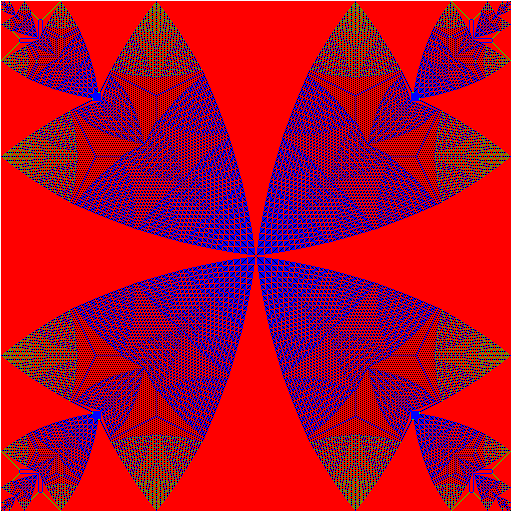
\includegraphics[width=1\linewidth]{dump-asandPile-seq-dim-512-iter-34938_default}
        \caption{\small{avec do\_tile\_default}}
        % \label{fig:asandPile_default}
    \end{subfigure}
    \begin{subfigure}{.4\textwidth}
        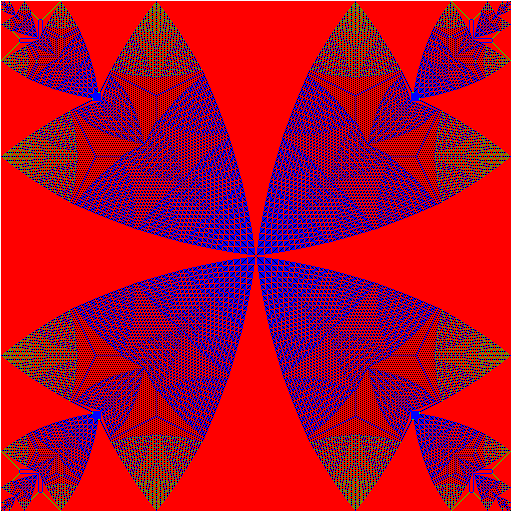
\includegraphics[width=1\linewidth]{dump-asandPile-seq-dim-512-iter-34938_opt}
        \caption{\small{avec do\_tile\_opt}}
        % \label{fig:asandPile_opt}
    \end{subfigure}
    \caption{Verification du résultats pour asandPile}
\end{figure}

Le gain de performance est de $1.2$ car $\frac{37990}{31405}$

\section{OpenMP implementation of the synchronous version (4.2)}

Pour \emph{ssandPile\_compute\_omp()} on a fait en sorte de partourir chaque grain de sable
puis on ajouter un \em{pragam omp for} pour que chaque grain de sable sois calculer par un thread.\\

Le code de la fonction :
\inputminted[
    frame=lines,
    framesep=2mm,
    baselinestretch=1.2,
    fontsize=\footnotesize,
    linenos
]{c}{codes/sync_omp.c}

Pour \emph{ssandPile\_compute\_omp\_tiled()} on a dupliquer la version tile pour y ajouter
un \em{pragam omp for} avec un \em{collapse(2)} pour que les tuiles soit calculer pars des threads.\\

% TODO: description taille de tuiles
\begin{figure}[H]
    \centering
    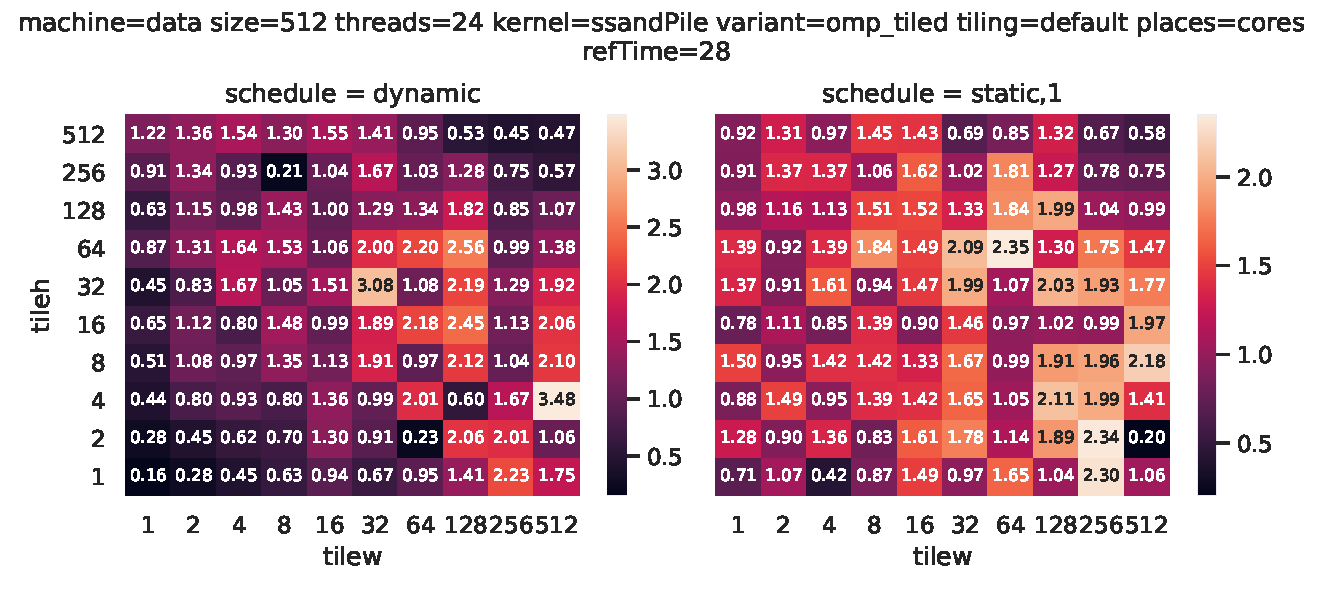
\includegraphics[width=1\linewidth]{ssand_omp_tiled}
\end{figure}

La heatmap montre que en moyenne, le schedule static est meilleur que le dynamique, 
cependant on cherche à resoudre un problème précis, donc on va chercher l'accélération maximale.
Ici ce sera avec des tuiles de width 512 et de height 4 en schedule dynamique.

% TODO: ssandPile_compute_omp_taskloop

\section{OpenMP implementation of the asynchronous version (4.3)}

Pour paralleliser avec \emph{asandPile\_compute\_omp\_tiled}, il a fallu créer 4 nids de boucles afin d'éviter les lectures/écritures concurentes.
On a donc un nid de boucle pour les lignes et colonnes impaires, 
un pour les lignes impaires et colonnes paires, 
un pour les lignes paires et colonnes impaires, 
et un pour les lignes et colonnes paires.

Le code de la fonction final :
\inputminted[
    frame=lines,
    framesep=2mm,
    baselinestretch=1.2,
    fontsize=\footnotesize,
    linenos,
    firstline=1,
    lastline=23
]{c}{codes/async_omp_tiled.c}
\emph{Le nid BLEU est répété 4 fois avec des initialisations de x et y qui diffèrent}

\begin{figure}[H]
    \centering
    \begin{subfigure}{.4\textwidth}
        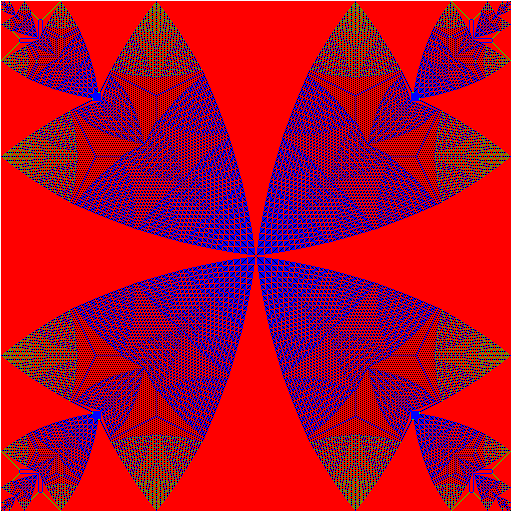
\includegraphics[width=1\linewidth]{dump-asandPile-seq-dim-512-iter-34938_default}
        \caption{\small{version seq}}
        % \label{fig:asandPile_default}
    \end{subfigure}
    \begin{subfigure}{.4\textwidth}
        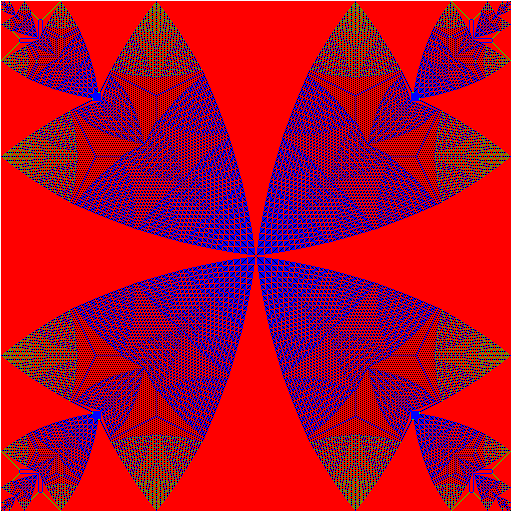
\includegraphics[width=1\linewidth]{dump-asandPile-omp_tiled-dim-512-iter-34954}
        \caption{\small{version omp\_tiled}}
        % \label{fig:asandPile_opt}
    \end{subfigure}
    \caption{Verification du résultats pour asandPile}
\end{figure}

Le gain de performance par rapport au séquentiel avec tuiles optimisées est de $1.98$ car $\frac{30927.379}{15641.740}$

\begin{figure}[H]
    \centering
    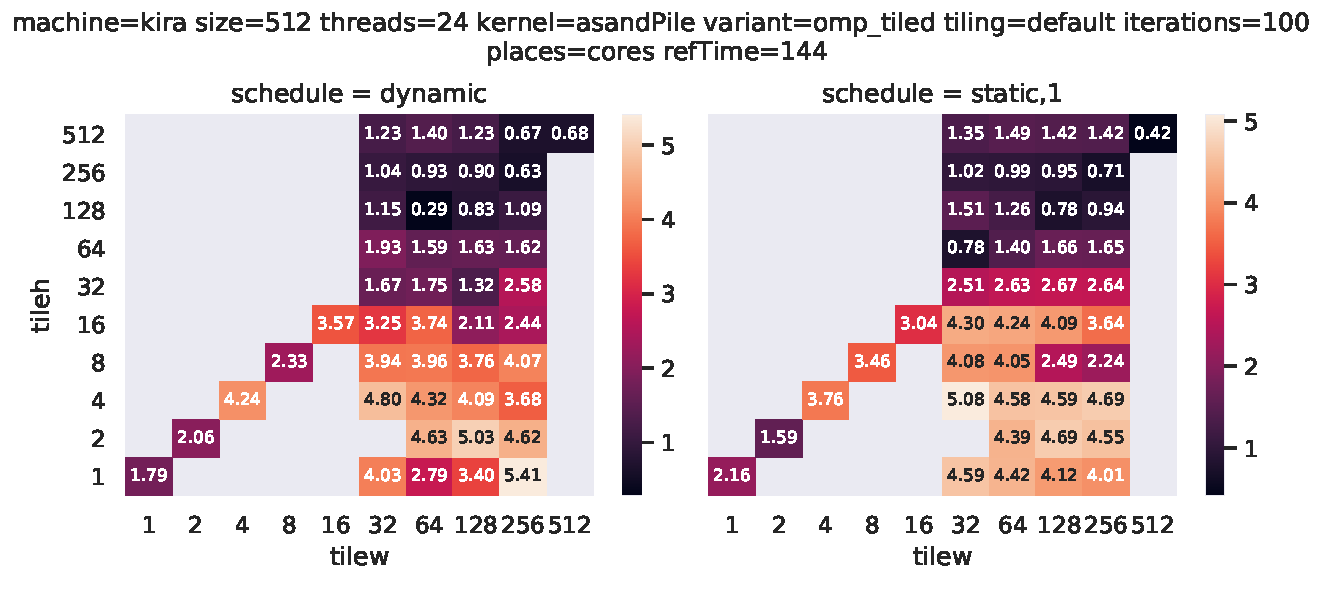
\includegraphics[width=1\linewidth]{Heatmap-asand_omp}
    \caption{\small{heatmap comparaison omp\_tiled \& tiled}}
    % \label{fig:heatmaplazy}
\end{figure}

Les expériences montrent que pour certaines tailles de tuiles, il n'y a pas de résultat d'accélération, et après vérification, le programme ne fonctionne pas sur ces tailles là.
Néanmoins, avec ces résultats, ont en déduit que le schedule static,1 avec une width de 32 et une height de 4 est la meilleure option.

% TODO: Then you can compare the performance of all variants on the size 512 case.
\begin{figure}[H]
    \centering
    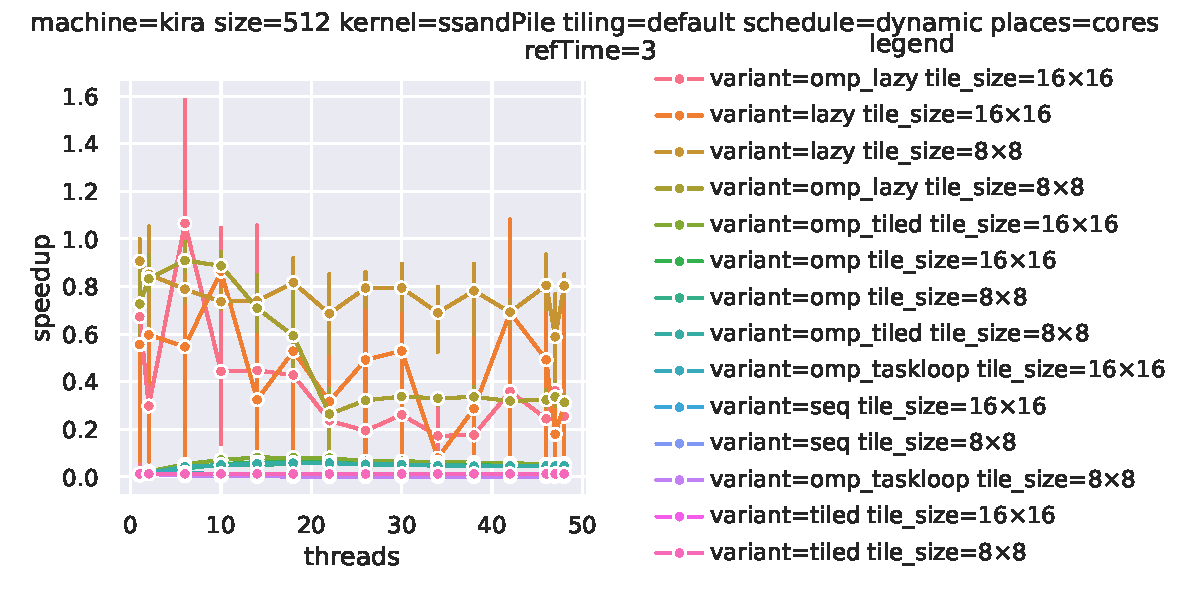
\includegraphics[width=1\linewidth]{ssand-xp-all_8_16.pdf}
    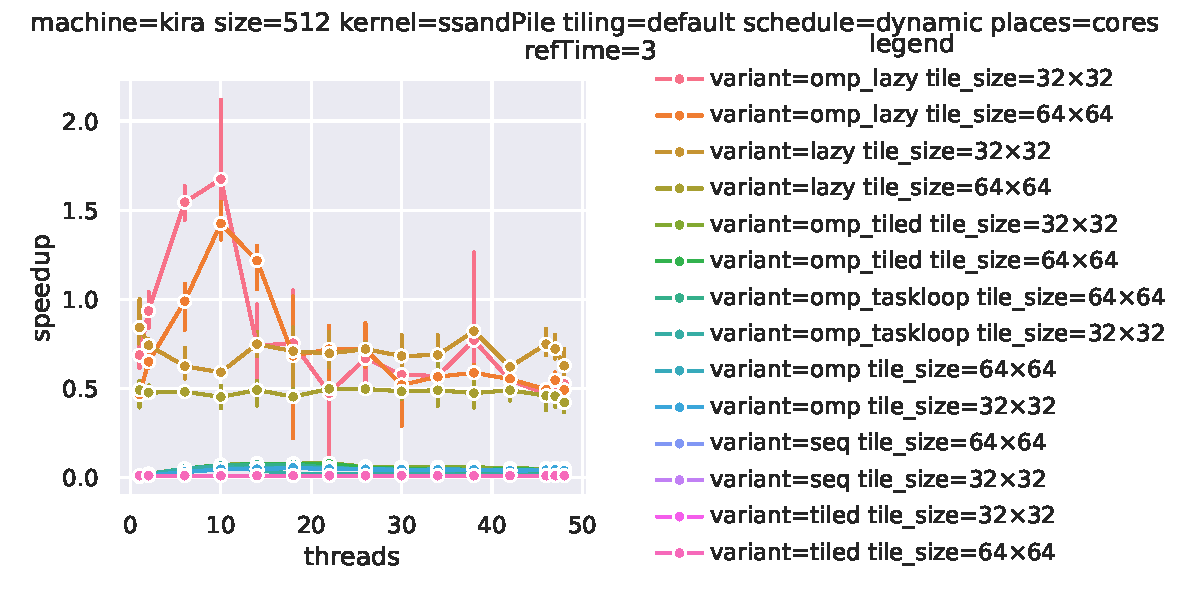
\includegraphics[width=1\linewidth]{ssand-xp-all_32_64.pdf}
    \caption{\small{ssandPile comparaison de toutes les variants}}
    % \label{fig:ssand-xp-all}
\end{figure}
\begin{figure}[H]
    \centering
    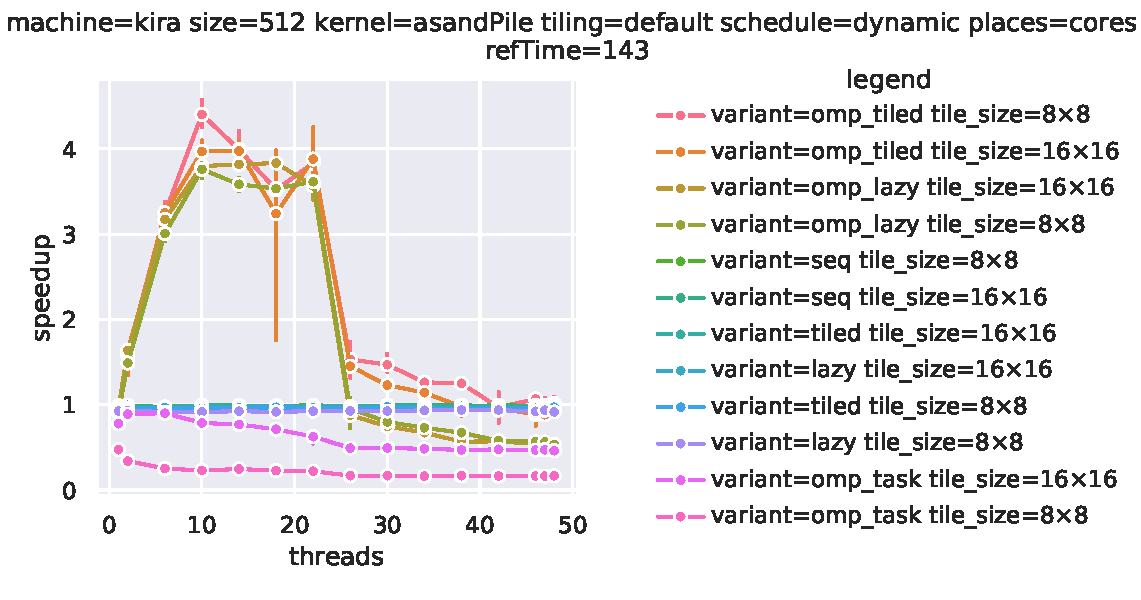
\includegraphics[width=1\linewidth]{asand-xp-all_8_16.pdf}
    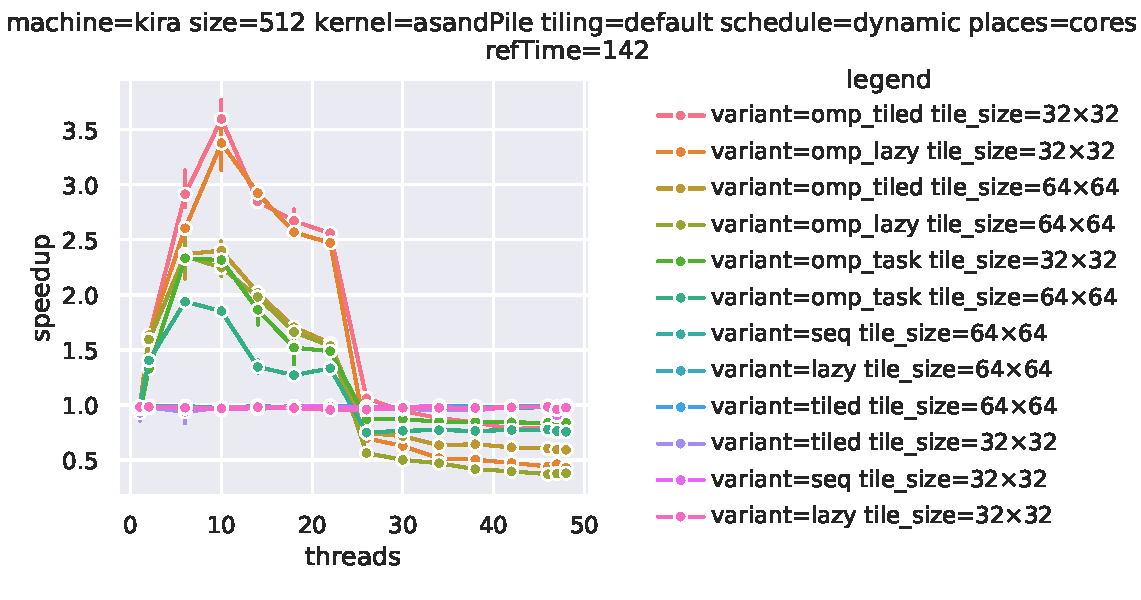
\includegraphics[width=1\linewidth]{asand-xp-all_32_64.pdf}
    \caption{\small{asandPile comparaison de toutes les variants}}
    % \label{fig:asand-xp-all}
\end{figure}

\section{Lazy OpenMP implementations (4.4)}

Pour la version asynchrone, nous avons repris la version précédente et ajouté deux tableaux
servant successivement de lecture et d'écriture pour tester si les tuiles autour ont été modifiés à l'itération précédente.

\begin{figure}[H]
    \centering
    \begin{subfigure}{.4\textwidth}
        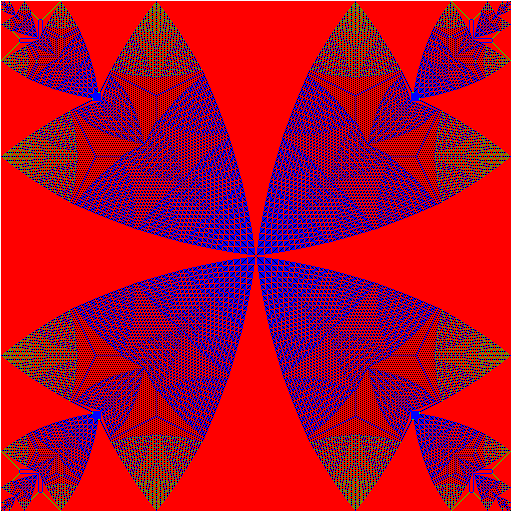
\includegraphics[width=1\linewidth]{dump-asandPile-seq-dim-512-iter-34938_default}
        \caption{\small{avec do\_tile\_default}}
        % \label{fig:asandPile_default}
    \end{subfigure}
    \begin{subfigure}{.4\textwidth}
        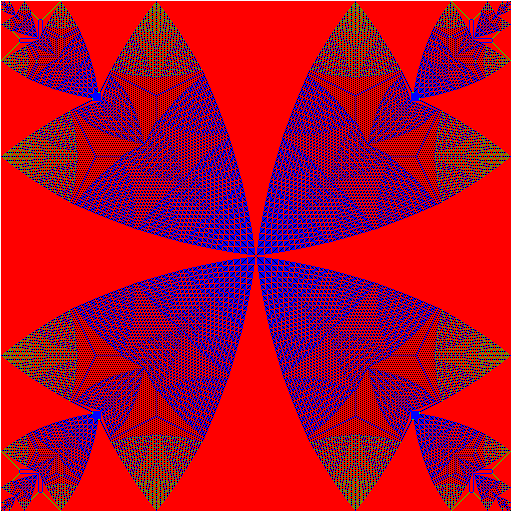
\includegraphics[width=1\linewidth]{dump-asandPile-omp_lazy-dim-512-iter-34954}
        \caption{\small{version omp\_lazy}}
        % \label{fig:asandPile_opt}
    \end{subfigure}
    \caption{Verification du résultats pour asandPile}
\end{figure}

Le gain de performance par rapport au asynchrone lazy avec tuiles optimisées est de $1.35$ car $\frac{32292.716}{23825.744}$

\begin{figure}[H]
    \centering
    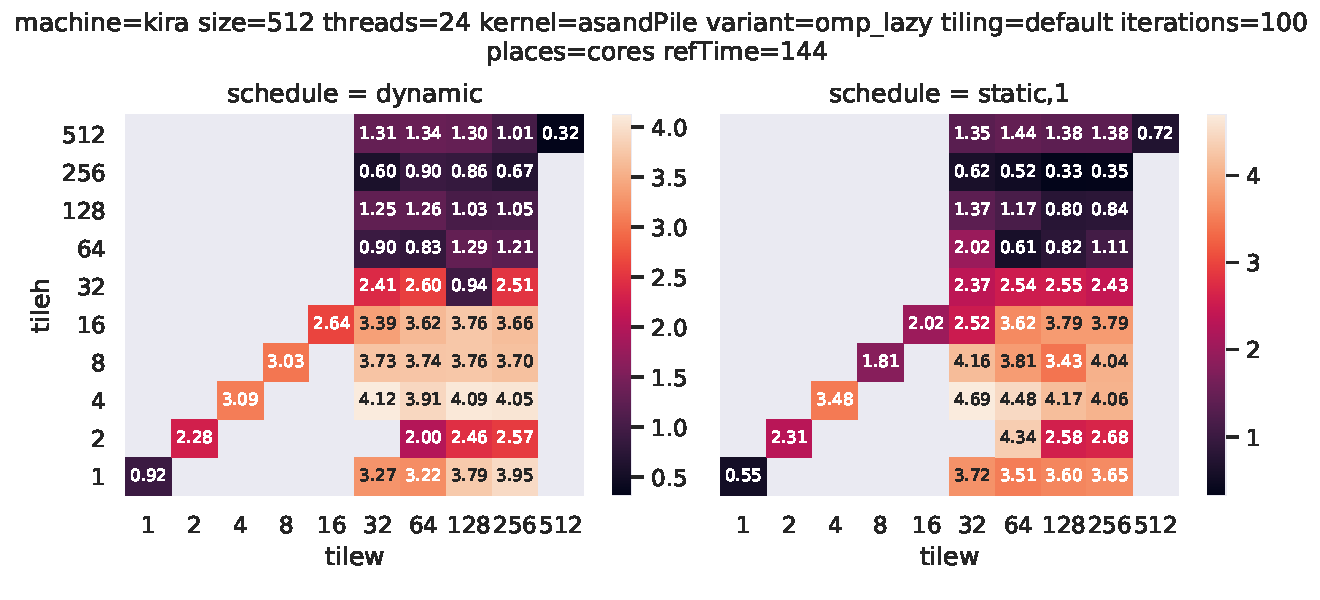
\includegraphics[width=1\linewidth]{Heatmap-asand_omp_lazy}
    \caption{\small{heatmap comparaison omp\_lazy \& lazy}}
    % \label{fig:heatmaplazy}
\end{figure}

Les expériences montrent que pour certaines tailles de tuiles, il n'y a pas de résultat d'accélération, et après vérification, le programme ne fonctionne pas sur ces tailles là.
Néanmoins, avec ces résultats, ont en déduit que le schedule static,1 avec une width de 32 et une height de 4 est la meilleure option.

\end{document}